\chapter{Perception of Rhetorical Tactics in Individual Comments}
\label{perception}

This chapter examines how the different types of argument discussed in the previous chapter are perceived by their audience. An experiment was carried out in which participants were shown a number of social media posts, and asked a series of questions (answerable on a Likert scale) about each one. These questions gauged both how they felt about the post (e.g. entertained or offended), and how they would act on it (e.g. replying or reporting).


\section{Methodology}

\subsection{Data Sample}
\label{perception:method:sample}

This work used the ``normal'' threads acquired in Section \ref{case:method:sample}.

Each of these ``normal'' threads was then annotated by topic, using one of the following categories based on an aggregation of the topics provided by the five news distribution sites the social media accounts of which the stories were sourced from:
\textit{Current Events}, stories covering recent or ongoing occurrences;
\textit{Business}, stories involving businesses and/or the economy;
\textit{Politics}, stories relating to politics, politicians, elections, etc.;
\textit{Science \& Technology}, stories relating to science, the environment, new technologies, etc.;
\textit{Entertainment \& Arts}, stories involving cultural events, celebrities, etc.;
\textit{Sports}, stories covering sporting events and participants;
and \textit{Features}, stories that form an opinion piece, or focus on an individual rather than the broader story they are a part of.


\begin{table}
\centering
\caption{Threads by topic}
\label{table:perception:topics}
\begin{tabular}{ l | l | l | l | l}
\textbf{Platform} & \textbf{Current Events} & \textbf{Business} & \textbf{Politics} & \textbf{Science \& Technology} \\
\hline
Facebook & 52 & 18 & 23 & 16 \\
\hline
Twitter & 53 & 3 & 24 & 12\\
\hline
Reddit & 41 & 4 & 2 & 6\\
\end{tabular}
\newline
\newline
\begin{tabular}{ l | l | l | l}
\textbf{Platform} & \textbf{Entertainment \& Arts} & \textbf{Sports} & \textbf{Feature}\\
\hline
Facebook & 20 & 3 & 32 \\
\hline
Twitter & 12 & 3 & 20 \\
\hline
Reddit & 2 & 0 & 0 \\
\end{tabular}
\end{table}
 

\subsection{Classifications}

\TODO{Argument}

\TODO{Social} 
 \citet{kietzmann2011social} describe seven
Identity, Sharing, Presence, Relationships, Reputation, Groups, and Conversations



Table \ref{table:perception:questions} summarises each of these classifications, and provides justification for their inclusion.

\subsection{Participants and Survey}
Participants were invited via a general call on social media; they were provided an information sheet and consent form, and asked to confirm that they were above the age of eighteen. Participants were shown a selection eighteen posts taken from the sample described in Section \ref{perception:method:sample} (three different news-types across three social media platforms). For context, they were also show the initial post in the thread and, if present, any post that was directly replied to by the target. These were presented to participants via a web-survey, a screenshot of which is shown in Figure \ref{figure:perception:survey}.

\begin{figure}
\centering
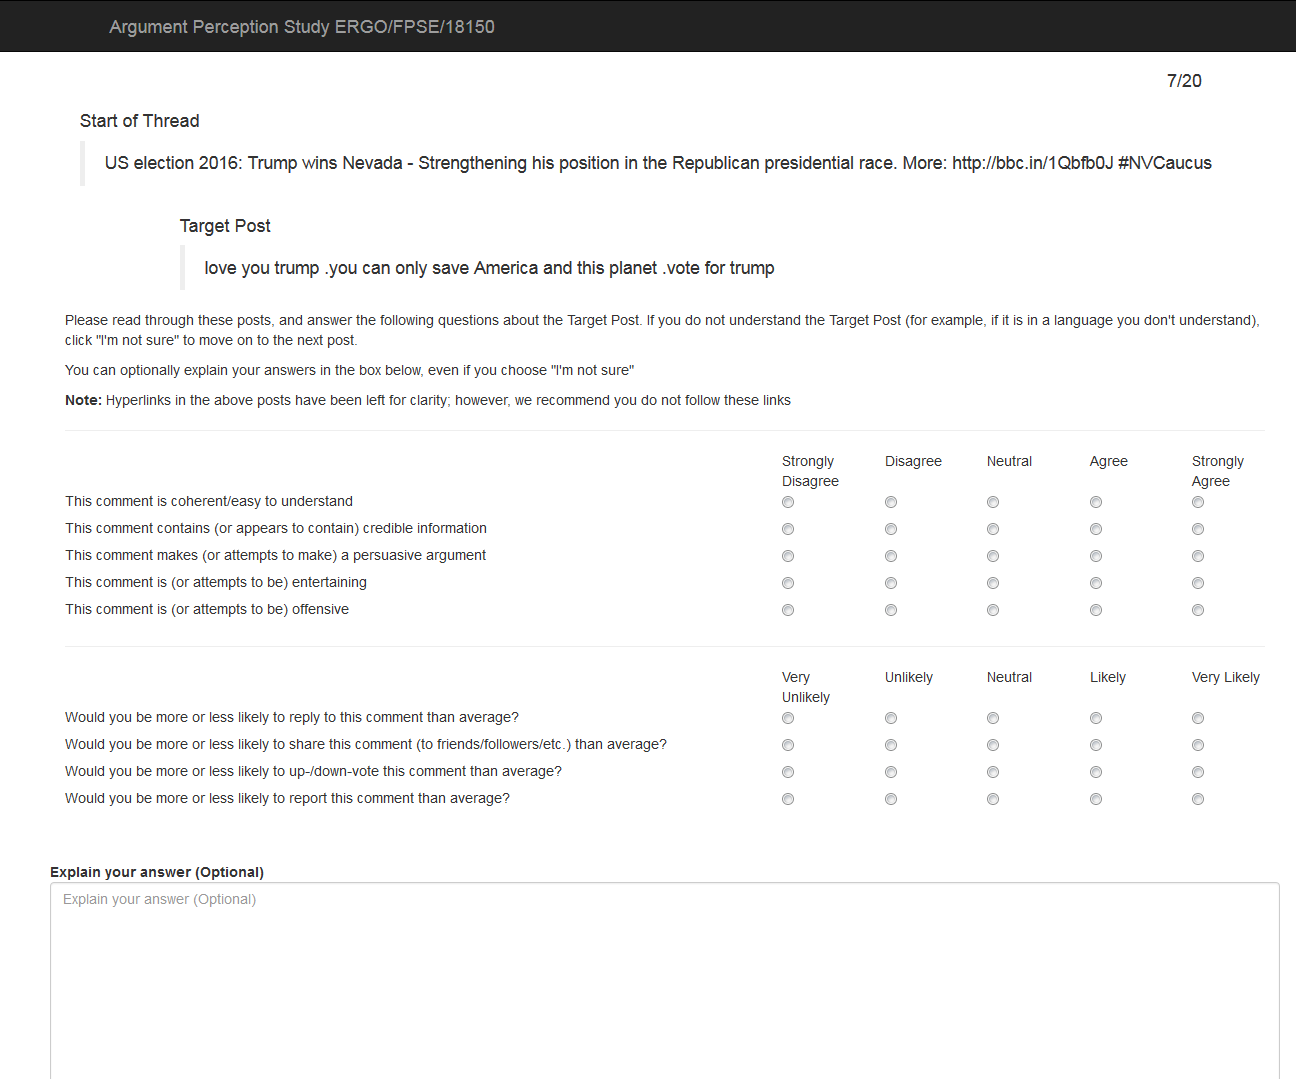
\includegraphics[scale=0.45]{perception/survey1.png}
\caption{The questionnaire as presented to participants}
\label{figure:perception:survey}
\end{figure}

Every participant was also shown, and asked to rate, two additional posts common to all participants to judge the overall inter-rater agreement. These were selected at random from the sampled pool of comments and manually inspected to ensure they were non-empty and comprehensible (e.g., English-language).

\begin{table}
\centering
\caption{Example classifications of argumentation posts}
\label{table:perception:questions}
\begin{tabular}{ l | p{10cm}}
\textbf{Factor} & \textbf{Description} \\
\hline
Coherence & Whether the post is clear and understandable \CITATION  \\
\hline
Credibility & Whether the post contains (purportedly) credible information \CITATION \\
\hline
Persuasiveness & Whether the post attempts to change the readers position \citep{sundar2000}\\
\hline
Entertainment & Whether the post engages or bores the reader \citep{sundar2000}\\
\hline
Offence & \\
\hline
Reply & How likely the reader is to reply\citep{markova2013} \citep{kietzmann2011social}\\
\hline
Share & \citep{markova2013} \citep{kietzmann2011social}\\
\hline
Vote & \citep{markova2013} \citep{kietzmann2011social}\\
\hline
Report &\citep{kietzmann2011social} \\

%Identity & \citep{kietzmann2011social}\\
%\hline
%Sharing & \citep{kietzmann2011social}\\
%\hline
%Presence & \citep{kietzmann2011social}\\
%\hline
%Relationships &\citep{kietzmann2011social} \\
%\hline
%Reputation & \citep{kietzmann2011social}\\
%\hline
%Groups & \citep{kietzmann2011social}\\
%\hline
%Conversations & \citep{kietzmann2011social}\\

\end{tabular}
\end{table}

\section{Data Analysis and Results}

\subsection{Raw Data}

Table \ref{table:perception:breakdown} shows the raw answers that participants gave to the questions overall. Even here, it is relatively easy to see (from questions 6-9) that the majority of people would not be inclined to interact or engage with the comments that were presented here. In addition to these results, 45 people skipped this question

\begin{table}
\centering
\caption{Breakdown of answers given for each question}
\label{table:perception:breakdown}
\begin{tabular}{ p{6cm} | r | r | r | r | r }
\textbf{Question} & \textbf{1} &  \textbf{2} &  \textbf{3} &  \textbf{4} &  \textbf{5}\\
\hline
This comment is coherent/easy to understand  &  48 & 134 & 71 & 374 & 119 \\
\hline
This comment contains (or appears to contain) credible information  &  127 & 230 & 224 & 133 & 32 \\
\hline
This comment makes (or attempts to make) a persuasive argument  &  111 & 172 & 159 & 252 & 52 \\
\hline
This comment is (or attempts to be) entertaining  &  126 & 189 & 151 & 220 & 60 \\
\hline
This comment is (or attempts to be) offensive  &  165 & 208 & 194 & 143 & 36 \\
\hline
Would you be more or less likely to reply to this comment than average?  &  232 & 216 & 183 & 108 & 7 \\
\hline
Would you be more or less likely to share this comment (to friends/followers/etc.) than average?  &  291 & 226 & 176 & 51 & 2 \\
\hline
Would you be more or less likely to up-/down-vote this comment than average?  &  207 & 179 & 195 & 143 & 22 \\
\hline
Would you be more or less likely to report this comment than average?  &  296 & 204 & 211 & 30 & 5 \\
\end{tabular}
\end{table}


Table \ref{table:perception:annotation-breakdown} shows the number of responses given per each different annotation type. Note that as a post may have multiple annotations, there may be (and is likely to be) overlap in the number of responses. From this we can see the distribution of annotations, combined with random selection and the ability of participants to skip questions, resulted in only one response for the \textit{Spam/Advertisement} category, and only two for the \textit{Preference} category. However, posts annotated as containing Logical Attack/Support and Rhetorical Attack/Support, the key element of this perception study, received over one hundred responses each.

\begin{table}
\centering
\caption{Number of responses given per annotation}
\label{table:perception:annotation-breakdown}
\begin{tabular}{ l | r }
\textbf{Annotation} & \pbox{2cm}{\textbf{Number of}\\\textbf{Responses}}\\
\hline
Information & 491\\
Transition & 40\\
Logical Attack & 146\\
Logical Support & 27\\
Rhetorical Attack & 256\\
Rhetorical Support & 181\\
Preference & 2\\
Entity & 307\\
Group & 55\\
Audience & 104\\
Implied Relationship & 7\\
Implied Belief & 30\\
Spam/Advertisement & 1\\	
Unknown & 4\\
None & 10\\
\end{tabular}
\end{table}


\subsection{Inter Rater Reliability}
\label{perception:results:interrater}
To gain an additional insight of how much agreement there was between participants, and if there was particularly strong areas of agreement or disagreement, the first and last statements shown were identical to all participants. These statements were selected at random from the sample pool, but were manually inspected to ensure they were non-empty and comprehensible (e.g., English-language).

The first post, taken from Reddit, reads as follows:
\textit{The FSA is also irrelevant. Nusra and/or ISIS would be be the rulers if Assad collapsed. And also, NO the ``FSA'' is mostly islamists, most of the ``secular rebels'' have switched around and have become part of the SDF which is part of the YPG.} This was annotated as having Information, and a Logical Attack. Table \ref{table:perception:first-raw} shows the raw answers that participants gave to the first question. In addition to these results, 10 people skipped this question. Table \ref{table:perception:first-averages} shows the distribution of these answers: while  there is a relatively large range between the minimum and maximum responses the standard deviation is not excessive. The largest value (1.218) was for the question \textit{This comment makes (or attempts to make) a persuasive argument.} The lowest values were for the questions exploring the perception of entertainment and credibility (0.764 and 0.899 respectively).


\begin{table}
\centering
\caption{Breakdown of answers given for the first question}
\label{table:perception:first-raw}
\begin{tabular}{ p{6cm} | r | r | r | r | r }
\textbf{Question} & \textbf{1} &  \textbf{2} &  \textbf{3} &  \textbf{4} &  \textbf{5}\\
\hline
This comment is coherent/easy to understand  &  6 & 23 & 8 & 16 & 2 \\
\hline
This comment contains (or appears to contain) credible information  &  4 & 18 & 22 & 10 & 1 \\
\hline
This comment makes (or attempts to make) a persuasive argument  &  7 & 11 & 8 & 24 & 5 \\
\hline
This comment is (or attempts to be) entertaining  &  26 & 23 & 4 & 2 & 0 \\
\hline
This comment is (or attempts to be) offensive  &  15 & 21 & 13 & 6 & 0 \\
\hline
Would you be more or less likely to reply to this comment than average?  &  19 & 15 & 11 & 10 & 0 \\
\hline
Would you be more or less likely to share this comment (to friends/followers/etc.) than average?  &  23 & 16 & 12 & 4 & 0 \\
\hline
Would you be more or less likely to up-/down-vote this comment than average?  &  14 & 17 & 15 & 9 & 0 \\
\hline
Would you be more or less likely to report this comment than average?  &  18 & 14 & 21 & 2 & 0 \\
\end{tabular}
\end{table}


\begin{table}
\centering
\caption{Distribution of answers given for the first question}
\label{table:perception:first-averages}
\begin{tabular}{ !p{3cm} | ^r | ^r | ^r | ^r | ^r | ^r | ^r}
\rowstyle{\bfseries} Question & Min. & \pbox{2cm}{Lower\\ Quartile} & Median & \pbox{2cm}{Upper\\ Quartile} & Max. & Mean & $\sigma$\\
\hline
This comment is coherent/easy to understand  &  1.00 & 2.00 & 2.00 & 4.00 & 5.00 & 2.727 & 1.103 \\
\hline
This comment contains (or appears to contain) credible information  &  1.00 & 2.00 & 3.00 & 3.00 & 5.00 & 2.745 & 0.899 \\
\hline
This comment makes (or attempts to make) a persuasive argument  &  1.00 & 2.00 & 4.00 & 4.00 & 5.00 & 3.164 & 1.218 \\
\hline
This comment is (or attempts to be) entertaining  &  1.00 & 1.00 & 2.00 & 2.00 & 4.00 & 1.673 & 0.764 \\
\hline
This comment is (or attempts to be) offensive  &  1.00 & 1.00 & 2.00 & 3.00 & 4.00 & 2.182 & 0.955 \\
\hline
Would you be more or less likely to reply to this comment than average?  &  1.00 & 1.00 & 2.00 & 3.00 & 4.00 & 2.218 & 1.107 \\
\hline
Would you be more or less likely to share this comment (to friends/followers/etc.) than average?  &  1.00 & 1.00 & 2.00 & 3.00 & 4.00 & 1.945 & 0.961 \\
\hline
Would you be more or less likely to up-/down-vote this comment than average?  &  1.00 & 1.50 & 2.00 & 3.00 & 4.00 & 2.345 & 1.031 \\
\hline
Would you be more or less likely to report this comment than average?  &  1.00 & 1.00 & 2.00 & 3.00 & 4.00 & 2.127 & 0.916 \\
\end{tabular}
\end{table}


The last post, taken from Twitter, reads as follows:
\textit{@steve\_walke23 @guardian @lisaocarroll Some beings are inhuman - ISIS atrocities don't bother you? Get off your priggish high horse.} This was annotated as having Information and a Rhetorical Attack, directed against an Entity (in this case likely representing one of @steve\_walke23 or @lisaocarroll, or potentially both).

Table \ref{table:perception:last-raw} shows the raw answers that participants gave to the last question. In addition to these results, 2 people skipped this question. Because fewer people completed every question of the survey, dropping out before the total number of responses to these questions is lower than that of the first post.

Table \ref{table:perception:last-averages} shows the distribution of these answers. The standard deviations are not widely different from the responses to the first group of questions in scale, though they do differ by question. The largest value (1.159), lower than the highest standard deviation of the first group of questions, was shared by the questions examining participants reactions, specifically replying to and voting on.

The lowest values (0.840 and 0.904 respectively), higher than the lowest standard deviations of the first group of questions, were in response to the likelihood participants would reply to this comment (the majority were in agreement that they would not) and judging whether it was considered coherent (on average, participants found it neither excessively clear or unclear).


\begin{table}
\centering
\caption{Breakdown of answers given for the last question}
\label{table:perception:last-raw}
\begin{tabular}{ p{6cm} | r | r | r | r | r }
\textbf{Question} & \textbf{1} &  \textbf{2} &  \textbf{3} &  \textbf{4} &  \textbf{5}\\
\hline
This comment is coherent/easy to understand  &  0 & 6 & 3 & 19 & 3 \\
\hline
This comment contains (or appears to contain) credible information  &  4 & 10 & 12 & 4 & 1 \\
\hline
This comment makes (or attempts to make) a persuasive argument  &  2 & 3 & 6 & 18 & 2 \\
\hline
This comment is (or attempts to be) entertaining  &  4 & 14 & 8 & 5 & 0 \\
\hline
This comment is (or attempts to be) offensive  &  1 & 4 & 3 & 17 & 6 \\
\hline
Would you be more or less likely to reply to this comment than average?  &  8 & 7 & 7 & 9 & 0 \\
\hline
Would you be more or less likely to share this comment (to friends/followers/etc.) than average?  &  11 & 12 & 7 & 1 & 0 \\
\hline
Would you be more or less likely to up-/down-vote this comment than average?  &  8 & 9 & 7 & 6 & 1 \\
\hline
Would you be more or less likely to report this comment than average?  &  10 & 8 & 12 & 1 & 0 \\
\end{tabular}
\end{table}


\begin{table}
\centering
\caption{Distribution of answers given for the last question}
\label{table:perception:last-averages}
\begin{tabular}{ !p{3cm} | ^r | ^r | ^r | ^r | ^r | ^r | ^r}
\rowstyle{\bfseries} Question & Min. & \pbox{2cm}{Lower\\ Quartile} & Median & \pbox{2cm}{Upper\\ Quartile} & Max. & Mean & $\sigma$\\
\hline
This comment is coherent/easy to understand  &  2.00 & 3.00 & 4.00 & 4.00 & 5.00 & 3.613 & 0.904 \\
\hline
This comment contains (or appears to contain) credible information  &  1.00 & 2.00 & 3.00 & 3.00 & 5.00 & 2.613 & 0.973 \\
\hline
This comment makes (or attempts to make) a persuasive argument  &  1.00 & 3.00 & 4.00 & 4.00 & 5.00 & 3.484 & 0.979 \\
\hline
This comment is (or attempts to be) entertaining  &  1.00 & 2.00 & 2.00 & 3.00 & 4.00 & 2.452 & 0.910 \\
\hline
This comment is (or attempts to be) offensive  &  1.00 & 3.50 & 4.00 & 4.00 & 5.00 & 3.742 & 1.015 \\
\hline
Would you be more or less likely to reply to this comment than average?  &  1.00 & 1.50 & 3.00 & 4.00 & 4.00 & 2.548 & 1.159 \\
\hline
Would you be more or less likely to share this comment (to friends/followers/etc.) than average?  &  1.00 & 1.00 & 2.00 & 2.50 & 4.00 & 1.935 & 0.840 \\
\hline
Would you be more or less likely to up-/down-vote this comment than average?  &  1.00 & 1.50 & 2.00 & 3.00 & 5.00 & 2.452 & 1.159 \\
\hline
Would you be more or less likely to report this comment than average?  &  1.00 & 1.00 & 2.00 & 3.00 & 4.00 & 2.129 & 0.907 \\
\end{tabular}
\end{table}

\subsection{Question Breakdown}
\label{perception:results:breakdown}
In this section, a summary of the responses to each of the questions is presented, compared against the annotations present on the post. Table \ref{table:perception:mean-summary-classification} shows the mean Likert values for each question, and Table \ref{table:perception:deviation-summary-classification} shows the standard deviation from this mean. The full results are presented in Appendix \ref{appendix:perception-data} (Tables \ref{table:perception:coherent-classification}-\ref{table:perception:report-classification}). Note that as a post may have multiple annotations, there may be (and is likely to be) overlap in the number of responses.  

\TODO{TALK ABOUT WHY THESE NUMBERS ARE INTERESTING}
Discounting posts that received few responses (e.g. Preferences and Spam/Advertisement) it can be seen that there is a reasonable level of variation between participants ($\sigma>1$). However, for when asked how likely they would be to share
%(Table \ref{table:perception:share-classification})
or report,
%(Table \ref{table:perception:report-classification}),
participants were in closer agreement, in both cases stating they would be less likely to engage than average.

%Table \ref{table:perception:coherent-classification} shows the breakdown of agreement to the statement \textit{This comment is coherent/easy to understand}.

\begin{table}
\centering
\caption{Mean rating for each question, compared with annotations present}
\label{table:perception:mean-summary-classification}
\begin{tabular}{ !l | ^r ^r ^r ^r ^r ^r ^r ^r ^r}
& \multicolumn{9}{c}{\textbf{Mean Response to Question}} \\
\rowstyle{\bfseries} Annotation & Q1 & Q2 & Q3 & Q4 & Q5 & Q6 & Q7 & Q8 & Q9\\
\hline
Information             & 3.475 & 2.756 & 3.196 & 2.678 & 2.556 & 2.322 & 2.045 & 2.497 & 1.986 \\
Transition              & 3.750 & 2.600 & 2.825 & 2.650 & 2.575 & 2.525 & 2.025 & 2.450 & 1.900 \\
Logical Attack          & 3.308 & 2.966 & 3.329 & 2.158 & 2.301 & 2.390 & 2.048 & 2.548 & 1.973 \\
Logical Support         & 3.778 & 2.815 & 3.000 & 2.704 & 2.963 & 2.185 & 2.000 & 2.333 & 2.074 \\
Rhetorical Attack       & 3.527 & 2.418 & 2.965 & 3.094 & 3.164 & 2.199 & 1.863 & 2.426 & 2.094 \\
Rhetorical Support      & 3.580 & 2.547 & 2.685 & 3.420 & 2.309 & 2.271 & 2.122 & 2.530 & 1.972 \\
Preference              & 3.000 & 2.000 & 3.500 & 3.500 & 3.000 & 2.000 & 2.000 & 2.000 & 2.500 \\
Entity                  & 3.511 & 2.427 & 2.886 & 3.280 & 2.853 & 2.238 & 2.010 & 2.463 & 2.042 \\
Group                   & 3.527 & 2.873 & 3.273 & 2.873 & 2.873 & 2.200 & 1.927 & 2.618 & 2.182 \\
Audience                & 3.510 & 2.356 & 2.596 & 3.740 & 2.817 & 2.385 & 2.269 & 2.625 & 2.154 \\
Implied Relationship    & 3.429 & 2.143 & 3.143 & 2.857 & 3.429 & 1.571 & 1.571 & 2.429 & 2.714 \\
Implied Belief          & 3.800 & 2.333 & 3.000 & 2.967 & 3.333 & 2.067 & 1.800 & 2.667 & 2.333 \\
Spam/Advertisement      & 1.000 & 1.000 & 1.000 & 1.000 & 1.000 & 1.000 & 1.000 & 4.000 & 5.000 \\
Unknown                 & 2.750 & 2.000 & 2.000 & 2.250 & 1.500 & 1.500 & 1.500 & 2.250 & 1.500 \\
None                    & 3.100 & 1.700 & 1.600 & 3.000 & 1.700 & 1.700 & 1.200 & 1.700 & 1.600 \\
\end{tabular}
\end{table}



\begin{table}
\centering
\caption{Standard deviation from mean for each question, compared with annotations present}
\label{table:perception:deviation-summary-classification}
\begin{tabular}{ !l | ^r ^r ^r ^r ^r ^r ^r ^r ^r }
& \multicolumn{9}{c}{\textbf{Standard Deviation from Mean Response to Question}} \\
\rowstyle{\bfseries} Annotation & Q1 & Q2 & Q3 & Q4 & Q5 & Q6 & Q7 & Q8 & Q9\\
\hline
Information             & 1.131 & 1.069 & 1.137 & 1.178 & 1.152 & 1.088 & 0.950 & 1.162 & 0.932 \\
Transition              & 1.112 & 1.091 & 1.138 & 1.216 & 1.181 & 1.072 & 0.961 & 1.094 & 0.970 \\
Logical Attack          & 1.191 & 1.036 & 1.211 & 1.090 & 1.088 & 1.161 & 1.016 & 1.188 & 0.958 \\
Logical Support         & 0.737 & 1.020 & 1.089 & 0.974 & 1.261 & 0.862 & 0.903 & 0.903 & 0.979 \\
Rhetorical Attack       & 1.107 & 1.043 & 1.160 & 1.221 & 1.141 & 1.062 & 0.906 & 1.190 & 0.996 \\
Rhetorical Support      & 1.113 & 1.084 & 1.192 & 1.142 & 1.104 & 1.061 & 1.033 & 1.149 & 0.960 \\
Preference              & 1.000 & 0.000 & 0.500 & 0.500 & 0.000 & 0.000 & 0.000 & 0.000 & 0.500 \\
Entity                  & 1.122 & 1.032 & 1.177 & 1.181 & 1.206 & 1.052 & 0.970 & 1.167 & 0.999 \\
Group                   & 1.126 & 1.113 & 1.242 & 1.207 & 1.192 & 1.051 & 0.912 & 1.168 & 1.011 \\
Audience                & 1.109 & 1.028 & 1.043 & 0.971 & 1.116 & 1.059 & 1.058 & 1.145 & 0.948 \\
Implied Relationship    & 0.728 & 0.639 & 1.245 & 0.833 & 1.178 & 0.728 & 0.728 & 1.498 & 1.385 \\
Implied Belief          & 1.108 & 1.135 & 1.155 & 1.303 & 1.135 & 0.892 & 0.792 & 1.164 & 1.043 \\
Spam/Advertisement      & 0.000 & 0.000 & 0.000 & 0.000 & 0.000 & 0.000 & 0.000 & 0.000 & 0.000 \\
Unknown                 & 1.479 & 1.000 & 1.000 & 0.829 & 0.866 & 0.866 & 0.866 & 1.299 & 0.866 \\
None                    & 1.578 & 1.100 & 0.917 & 1.483 & 0.900 & 1.100 & 0.600 & 1.100 & 1.020 \\
\end{tabular}
\end{table}

\subsection{Logic/Rhetoric}
\label{perception:results:logic-rhetoric}
This section, and Tables \ref{table:perception:coherent-logic-rhetoric}-\ref{table:perception:report-logic-rhetoric}, examine how perception of arguments differ purely with regards to logical and rhetorical annotations (both attack and support). All other classifications are ignored for these tables.

Perhaps surprisingly, the majority of responses are very close, differing by a mean of \textless0.5. The largest difference was in response to whether the post was considered entertaining, with people considering rhetoric to be more entertaining by a margin of 0.967 (which was below the standard deviation). To determine if these observations can  be explained by the spread of different types of argument \textit{within} the umbrellas of logic and rhetoric, such as support and attack, these are considered in the next section.


\begin{table}
\centering
\caption{Average agreement with the statement \textit{This comment is coherent/easy to understand}, grouped by Logic and Rhetoric}
\label{table:perception:coherent-logic-rhetoric}
\begin{tabular}{ !l | ^r ^r ^r ^r ^r ^r ^r}
\rowstyle{\bfseries} Annotation & Min. & \pbox{2cm}{Lower\\ Quartile} & Median & \pbox{2cm}{Upper\\ Quartile} & Max. & Mean & $\sigma$\\
\hline
Logic  &  1.00 & 2.00 & 4.00 & 4.00 & 5.00 & 3.374 & 1.150 \\
Rhetoric  &  1.00 & 3.00 & 4.00 & 4.00 & 5.00 & 3.572 & 1.107 \\
\end{tabular}
\end{table}


\begin{table}
\centering
\caption{Average agreement with the statement \textit{This comment contains (or appears to contain) credible information}, grouped by Logic and Rhetoric}
\label{table:perception:credible-logic-rhetoric}
\begin{tabular}{ !l | ^r ^r ^r ^r ^r ^r ^r}
\rowstyle{\bfseries} Annotation & Min. & \pbox{2cm}{Lower\\ Quartile} & Median & \pbox{2cm}{Upper\\ Quartile} & Max. & Mean & $\sigma$\\
\hline
Logic  &  1.00 & 2.00 & 3.00 & 4.00 & 5.00 & 2.959 & 1.028 \\
Rhetoric  &  1.00 & 2.00 & 2.00 & 3.00 & 5.00 & 2.455 & 1.060 \\
\end{tabular}
\end{table}


\begin{table}
\centering
\caption{Average agreement with the statement \textit{This comment makes (or attempts to make) a persuasive argument}, grouped by Logic and Rhetoric}
\label{table:perception:persuasive-logic-rhetoric}
\begin{tabular}{ !l | ^r ^r ^r ^r ^r ^r ^r}
\rowstyle{\bfseries} Annotation & Min. & \pbox{2cm}{Lower\\ Quartile} & Median & \pbox{2cm}{Upper\\ Quartile} & Max. & Mean & $\sigma$\\
\hline
Logic  &  1.00 & 2.00 & 4.00 & 4.00 & 5.00 & 3.298 & 1.189 \\
Rhetoric  &  1.00 & 2.00 & 3.00 & 4.00 & 5.00 & 2.848 & 1.191 \\
\end{tabular}
\end{table}


\begin{table}
\centering
\caption{Average agreement with the statement \textit{This comment is (or attempts to be) entertaining}, grouped by Logic and Rhetoric}
\label{table:perception:entertaining-logic-rhetoric}
\begin{tabular}{ !l | ^r ^r ^r ^r ^r ^r ^r}
\rowstyle{\bfseries} Annotation & Min. & \pbox{2cm}{Lower\\ Quartile} & Median & \pbox{2cm}{Upper\\ Quartile} & Max. & Mean & $\sigma$\\
\hline
Logic  &  1.00 & 1.00 & 2.00 & 3.00 & 5.00 & 2.228 & 1.087 \\
Rhetoric  &  1.00 & 2.00 & 3.00 & 4.00 & 5.00 & 3.195 & 1.211 \\
\end{tabular}
\end{table}


\begin{table}
\centering
\caption{Average agreement with the statement \textit{This comment is (or attempts to be) offensive}, grouped by Logic and Rhetoric}
\label{table:perception:offensive-logic-rhetoric}
\begin{tabular}{ !l | ^r ^r ^r ^r ^r ^r ^r}
\rowstyle{\bfseries} Annotation & Min. & \pbox{2cm}{Lower\\ Quartile} & Median & \pbox{2cm}{Upper\\ Quartile} & Max. & Mean & $\sigma$\\
\hline
Logic  &  1.00 & 1.50 & 2.00 & 3.00 & 5.00 & 2.404 & 1.137 \\
Rhetoric  &  1.00 & 2.00 & 3.00 & 4.00 & 5.00 & 2.830 & 1.215 \\
\end{tabular}
\end{table}


\begin{table}
\centering
\caption{Average response to the question \textit{Would you be more or less likely to reply to this comment than average?}, grouped by Logic and Rhetoric}
\label{table:perception:reply-logic-rhetoric}
\begin{tabular}{ !l | ^r ^r ^r ^r ^r ^r ^r}
\rowstyle{\bfseries} Annotation & Min. & \pbox{2cm}{Lower\\ Quartile} & Median & \pbox{2cm}{Upper\\ Quartile} & Max. & Mean & $\sigma$\\
\hline
Logic  &  1.00 & 1.00 & 2.00 & 3.00 & 5.00 & 2.368 & 1.123 \\
Rhetoric  &  1.00 & 1.00 & 2.00 & 3.00 & 5.00 & 2.200 & 1.054 \\
\end{tabular}
\end{table}


\begin{table}
\centering
\caption{Average response to the question \textit{Would you be more or less likely to share this comment (to friends/followers/etc.) than average?}, grouped by Logic and Rhetoric}
\label{table:perception:share-logic-rhetoric}
\begin{tabular}{ !l | ^r ^r ^r ^r ^r ^r ^r}
\rowstyle{\bfseries} Annotation & Min. & \pbox{2cm}{Lower\\ Quartile} & Median & \pbox{2cm}{Upper\\ Quartile} & Max. & Mean & $\sigma$\\
\hline
Logic  &  1.00 & 1.00 & 2.00 & 3.00 & 5.00 & 2.047 & 1.002 \\
Rhetoric  &  1.00 & 1.00 & 2.00 & 3.00 & 4.00 & 1.938 & 0.953 \\
\end{tabular}
\end{table}


\begin{table}
\centering
\caption{Average response to the question \textit{Would you be more or less likely to up-/down-vote this comment than average?}, grouped by Logic and Rhetoric}
\label{table:perception:vote-logic-rhetoric}
\begin{tabular}{ !l | ^r ^r ^r ^r ^r ^r ^r}
\rowstyle{\bfseries} Annotation & Min. & \pbox{2cm}{Lower\\ Quartile} & Median & \pbox{2cm}{Upper\\ Quartile} & Max. & Mean & $\sigma$\\
\hline
Logic  &  1.00 & 1.50 & 3.00 & 3.00 & 5.00 & 2.520 & 1.151 \\
Rhetoric  &  1.00 & 1.00 & 2.00 & 3.00 & 5.00 & 2.473 & 1.185 \\
\end{tabular}
\end{table}


\begin{table}
\centering
\caption{Average response to the question \textit{Would you be more or less likely to report this comment than average?}, grouped by Logic and Rhetoric}
\label{table:perception:report-logic-rhetoric}
\begin{tabular}{ !l | ^r ^r ^r ^r ^r ^r ^r}
\rowstyle{\bfseries} Annotation & Min. & \pbox{2cm}{Lower\\ Quartile} & Median & \pbox{2cm}{Upper\\ Quartile} & Max. & Mean & $\sigma$\\
\hline
Logic  &  1.00 & 1.00 & 2.00 & 3.00 & 5.00 & 1.994 & 0.964 \\
Rhetoric  &  1.00 & 1.00 & 2.00 & 3.00 & 5.00 & 2.045 & 0.986 \\
\end{tabular}
\end{table}

\subsection{Support/Attack}
\label{perception:results:support-attack}
As noted in Section \ref{perception:results:logic-rhetoric}, there are different purposes for using logic or rhetoric that may account of the homogeneous results observed. By further breaking the answers down into different types of logic and rhetoric (specifically, support and attack) Tables \ref{table:perception:coherent-support-attack}-\ref{table:perception:report-support-attack} examine how perception varies further.

%Perhaps surprisingly, the majority of responses are very close, differing by a mean of <0.5. The largest difference was in response to whether the post was considered entertaining, with 0.967 (which was below the standard deviation). These observations can likely be explained by the spread of different types of argument \textit{within} the umbrellas of logic and rhetoric, such as support and attack which are considered in the next section.


Once more, the majority of responses are relatively close, differing by a mean of \textless0.5. Again the exception to this was whether posts was considered entertaining and, to a lesser degree, offensive. 

Supportive posts were considered to be more entertaining (by an average of 0.716) when using rhetorical devices rather than logical devices. They were also considered to be more offensive (by an average of 0.654) when using logical devices rather than rhetorical devices.

Attacking posts showed an even greater difference in opinion, with rhetorical posts being considered both more entertaining and more offensive (by a margin of 0.936 and 0.863 respectively) than logical posts.


\begin{table}
\centering
\caption{Average agreement with the statement \textit{This comment is coherent/easy to understand}, grouped by support and attack}
\label{table:perception:coherent-support-attack}
\begin{tabular}{ !l | ^r ^r ^r ^r ^r ^r ^r}
\rowstyle{\bfseries} Annotation & Min. & \pbox{2cm}{Lower\\ Quartile} & Median & \pbox{2cm}{Upper\\ Quartile} & Max. & Mean & $\sigma$\\
\hline
\rowstyle{\bfseries} Support  &  1.00 & 3.00 & 4.00 & 4.00 & 5.00 & 3.603 & 1.082 \\
Logical Support  &  2.00 & 3.50 & 4.00 & 4.00 & 5.00 & 3.778 & 0.737 \\
Rhetorical Support  &  1.00 & 3.00 & 4.00 & 4.00 & 5.00 & 3.580 & 1.113 \\
\rowstyle{\bfseries} Attack  &  1.00 & 2.00 & 4.00 & 4.00 & 5.00 & 3.445 & 1.140 \\
Logical Attack  &  1.00 & 2.00 & 4.00 & 4.00 & 5.00 & 3.308 & 1.191 \\
Rhetorical Attack  &  1.00 & 3.00 & 4.00 & 4.00 & 5.00 & 3.527 & 1.107 \\
\end{tabular}
\end{table}


\begin{table}
\centering
\caption{Average agreement with the statement \textit{This comment contains (or appears to contain) credible information}, grouped by support and attack}
\label{table:perception:credible-support-attack}
\begin{tabular}{ !l | ^r ^r ^r ^r ^r ^r ^r}
\rowstyle{\bfseries} Annotation & Min. & \pbox{2cm}{Lower\\ Quartile} & Median & \pbox{2cm}{Upper\\ Quartile} & Max. & Mean & $\sigma$\\
\hline
\rowstyle{\bfseries} Support  &  1.00 & 2.00 & 2.50 & 3.00 & 5.00 & 2.564 & 1.081 \\
Logical Support  &  1.00 & 2.00 & 3.00 & 3.50 & 5.00 & 2.815 & 1.020 \\
Rhetorical Support  &  1.00 & 2.00 & 3.00 & 3.00 & 5.00 & 2.547 & 1.084 \\
\rowstyle{\bfseries} Attack  &  1.00 & 2.00 & 3.00 & 3.00 & 5.00 & 2.613 & 1.074 \\
Logical Attack  &  1.00 & 2.00 & 3.00 & 4.00 & 5.00 & 2.966 & 1.036 \\
Rhetorical Attack  &  1.00 & 2.00 & 2.00 & 3.00 & 5.00 & 2.418 & 1.043 \\
\end{tabular}
\end{table}


\begin{table}
\centering
\caption{Average agreement with the statement \textit{This comment makes (or attempts to make) a persuasive argument}, grouped by support and attack}
\label{table:perception:persuasive-support-attack}
\begin{tabular}{ !l | ^r ^r ^r ^r ^r ^r ^r}
\rowstyle{\bfseries} Annotation & Min. & \pbox{2cm}{Lower\\ Quartile} & Median & \pbox{2cm}{Upper\\ Quartile} & Max. & Mean & $\sigma$\\
\hline
\rowstyle{\bfseries} Support  &  1.00 & 2.00 & 3.00 & 4.00 & 5.00 & 2.701 & 1.181 \\
Logical Support  &  1.00 & 2.00 & 3.00 & 4.00 & 4.00 & 3.000 & 1.089 \\
Rhetorical Support  &  1.00 & 2.00 & 3.00 & 4.00 & 5.00 & 2.685 & 1.192 \\
\rowstyle{\bfseries} Attack  &  1.00 & 2.00 & 3.00 & 4.00 & 5.00 & 3.082 & 1.201 \\
Logical Attack  &  1.00 & 2.00 & 4.00 & 4.00 & 5.00 & 3.329 & 1.211 \\
Rhetorical Attack  &  1.00 & 2.00 & 3.00 & 4.00 & 5.00 & 2.965 & 1.160 \\
\end{tabular}
\end{table}


\begin{table}
\centering
\caption{Average agreement with the statement \textit{This comment is (or attempts to be) entertaining}, grouped by support and attack}
\label{table:perception:entertaining-support-attack}
\begin{tabular}{ !l | ^r ^r ^r ^r ^r ^r ^r}
\rowstyle{\bfseries} Annotation & Min. & \pbox{2cm}{Lower\\ Quartile} & Median & \pbox{2cm}{Upper\\ Quartile} & Max. & Mean & $\sigma$\\
\hline
\rowstyle{\bfseries} Support  &  1.00 & 3.00 & 4.00 & 4.00 & 5.00 & 3.328 & 1.148 \\
Logical Support  &  1.00 & 2.00 & 3.00 & 3.00 & 5.00 & 2.704 & 0.974 \\
Rhetorical Support  &  1.00 & 3.00 & 4.00 & 4.00 & 5.00 & 3.420 & 1.142 \\
\rowstyle{\bfseries} Attack  &  1.00 & 2.00 & 3.00 & 4.00 & 5.00 & 2.753 & 1.257 \\
Logical Attack  &  1.00 & 1.00 & 2.00 & 3.00 & 5.00 & 2.158 & 1.090 \\
Rhetorical Attack  &  1.00 & 2.00 & 3.00 & 4.00 & 5.00 & 3.094 & 1.221 \\
\end{tabular}
\end{table}


\begin{table}
\centering
\caption{Average agreement with the statement \textit{This comment is (or attempts to be) offensive}, grouped by support and attack}
\label{table:perception:offensive-support-attack}
\begin{tabular}{ !l | ^r ^r ^r ^r ^r ^r ^r}
\rowstyle{\bfseries} Annotation & Min. & \pbox{2cm}{Lower\\ Quartile} & Median & \pbox{2cm}{Upper\\ Quartile} & Max. & Mean & $\sigma$\\
\hline
\rowstyle{\bfseries} Support  &  1.00 & 1.00 & 2.00 & 3.00 & 5.00 & 2.363 & 1.127 \\
Logical Support  &  1.00 & 2.00 & 3.00 & 4.00 & 5.00 & 2.963 & 1.261 \\
Rhetorical Support  &  1.00 & 1.00 & 2.00 & 3.00 & 5.00 & 2.309 & 1.104 \\
\rowstyle{\bfseries} Attack  &  1.00 & 2.00 & 3.00 & 4.00 & 5.00 & 2.839 & 1.189 \\
Logical Attack  &  1.00 & 1.00 & 2.00 & 3.00 & 5.00 & 2.301 & 1.088 \\
Rhetorical Attack  &  1.00 & 2.00 & 3.00 & 4.00 & 5.00 & 3.164 & 1.141 \\
\end{tabular}
\end{table}


\begin{table}
\centering
\caption{Average response to the question \textit{Would you be more or less likely to reply to this comment than average?}, grouped by support and attack}
\label{table:perception:reply-support-attack}
\begin{tabular}{ !l | ^r ^r ^r ^r ^r ^r ^r}
\rowstyle{\bfseries} Annotation & Min. & \pbox{2cm}{Lower\\ Quartile} & Median & \pbox{2cm}{Upper\\ Quartile} & Max. & Mean & $\sigma$\\
\hline
\rowstyle{\bfseries} Support  &  1.00 & 1.00 & 2.00 & 3.00 & 5.00 & 2.265 & 1.038 \\
Logical Support  &  1.00 & 1.50 & 2.00 & 3.00 & 4.00 & 2.185 & 0.862 \\
Rhetorical Support  &  1.00 & 1.00 & 2.00 & 3.00 & 5.00 & 2.271 & 1.061 \\
\rowstyle{\bfseries} Attack  &  1.00 & 1.00 & 2.00 & 3.00 & 5.00 & 2.295 & 1.106 \\
Logical Attack  &  1.00 & 1.00 & 2.00 & 3.00 & 5.00 & 2.390 & 1.161 \\
Rhetorical Attack  &  1.00 & 1.00 & 2.00 & 3.00 & 5.00 & 2.199 & 1.062 \\
\end{tabular}
\end{table}


\begin{table}
\centering
\caption{Average response to the question \textit{Would you be more or less likely to share this comment (to friends/followers/etc.) than average?}, grouped by support and attack}
\label{table:perception:share-support-attack}
\begin{tabular}{ !l | ^r ^r ^r ^r ^r ^r ^r}
\rowstyle{\bfseries} Annotation & Min. & \pbox{2cm}{Lower\\ Quartile} & Median & \pbox{2cm}{Upper\\ Quartile} & Max. & Mean & $\sigma$\\
\hline
\rowstyle{\bfseries} Support  &  1.00 & 1.00 & 2.00 & 3.00 & 4.00 & 2.108 & 1.019 \\
Logical Support  &  1.00 & 1.00 & 2.00 & 3.00 & 4.00 & 2.000 & 0.903 \\
Rhetorical Support  &  1.00 & 1.00 & 2.00 & 3.00 & 4.00 & 2.122 & 1.033 \\
\rowstyle{\bfseries} Attack  &  1.00 & 1.00 & 2.00 & 3.00 & 5.00 & 1.953 & 0.956 \\
Logical Attack  &  1.00 & 1.00 & 2.00 & 3.00 & 5.00 & 2.048 & 1.016 \\
Rhetorical Attack  &  1.00 & 1.00 & 2.00 & 2.00 & 4.00 & 1.863 & 0.906 \\
\end{tabular}
\end{table}


\begin{table}
\centering
\caption{Average response to the question \textit{Would you be more or less likely to up-/down-vote this comment than average?}, grouped by support and attack}
\label{table:perception:vote-support-attack}
\begin{tabular}{ !l | ^r ^r ^r ^r ^r ^r ^r}
\rowstyle{\bfseries} Annotation & Min. & \pbox{2cm}{Lower\\ Quartile} & Median & \pbox{2cm}{Upper\\ Quartile} & Max. & Mean & $\sigma$\\
\hline
\rowstyle{\bfseries} Support  &  1.00 & 2.00 & 3.00 & 3.00 & 5.00 & 2.505 & 1.122 \\
Logical Support  &  1.00 & 2.00 & 2.00 & 3.00 & 4.00 & 2.333 & 0.903 \\
Rhetorical Support  &  1.00 & 2.00 & 3.00 & 3.00 & 5.00 & 2.530 & 1.149 \\
\rowstyle{\bfseries} Attack  &  1.00 & 1.00 & 2.00 & 3.00 & 5.00 & 2.479 & 1.175 \\
Logical Attack  &  1.00 & 1.00 & 3.00 & 4.00 & 5.00 & 2.548 & 1.188 \\
Rhetorical Attack  &  1.00 & 1.00 & 2.00 & 3.00 & 5.00 & 2.426 & 1.190 \\
\end{tabular}
\end{table}


\begin{table}
\centering
\caption{Average response to the question \textit{Would you be more or less likely to report this comment than average?}, grouped by support and attack}
\label{table:perception:report-support-attack}
\begin{tabular}{ !l | ^r ^r ^r ^r ^r ^r ^r}
\rowstyle{\bfseries} Annotation & Min. & \pbox{2cm}{Lower\\ Quartile} & Median & \pbox{2cm}{Upper\\ Quartile} & Max. & Mean & $\sigma$\\
\hline
\rowstyle{\bfseries} Support  &  1.00 & 1.00 & 2.00 & 3.00 & 5.00 & 1.975 & 0.957 \\
Logical Support  &  1.00 & 1.00 & 2.00 & 3.00 & 4.00 & 2.074 & 0.979 \\
Rhetorical Support  &  1.00 & 1.00 & 2.00 & 3.00 & 5.00 & 1.972 & 0.960 \\
\rowstyle{\bfseries} Attack  &  1.00 & 1.00 & 2.00 & 3.00 & 5.00 & 2.050 & 0.968 \\
Logical Attack  &  1.00 & 1.00 & 2.00 & 3.00 & 5.00 & 1.973 & 0.958 \\
Rhetorical Attack  &  1.00 & 1.00 & 2.00 & 3.00 & 5.00 & 2.094 & 0.996 \\
\end{tabular}
\end{table}

\subsection{Rationale}
\label{perception:results:rationale}
Participants were provided a free-text area to optionally provide the reasons behind the choices they made. Below is a selection of these responses, their accompanying posts, and a discussion of what this means relating to the overall results noted above.




\TODO{Coherent}


Participants noted some of the features that they felt made an argument seem credible: either using direct quotes, or deliberately stating that the view was an opinion.

\textit{``Seems like a credible argument by using a quote''}

\textit{``...they're talking about their own opinions so it is credible.''}

Interestingly, participants often remarked that posts they had answered \textit{attempting} to persuade, did not strike them as particularly persuasive:




\TODO{entertaining}

Unsurprisingly, participants broadly felt that posts with foul language were offensive (although this was subjective), or those that directly insulted a person (whether within the discussion, or the topic of it), and often branded them as deliberate trolls. However, in certain cases, participants felt this would actually spur them to reply and engage with the discussion.

\textit{It's mildly offensive, but mostly it's just a bad, totally pointless joke, best ignored.}

\textit{It's just swearing so not particularly offensive.}

\textit{``I don't engage with racial hatred discussions. There's no rational discussion.''}

\textit{``The answer is trolling. Don't feed trolls.''}

\textit{``Essentially a trolling answer.''}

\textit{People are facing execution, and someone posts a dumb joke? It would be pretty funny in other contexts, but this is gross. I'd be more likely to reply just to call them out for being an ass.}


Participants had different opinions on how emotional language would change their behaviour; one explained that they were more likely to reply to posts that didn't seem emotionally charged, whereas another felt the opposite.

\textit{``I liked the non-emotional tone. So I would comfortable replying. But because my emotions are not engaged, I am less inclined to share''}

\textit{``It is emotionally engaging so prompts replying. It is entertaining that promots} [sic] \textit{sharing.''} 

There was also a relatively consistent consensus that participants were more likely to find a post persuasive, or vote for content, if they personally agreed with:

\textit{``The bias is: I am much more likely to share/upvote a comment if I agree with its contents.''}

\textit{``...Since I agree with the comment, I'm likely for me to vote up...''}

\textit{``...I tend to upvote content that I agree with and share content I disagree with...''}

As might be expected, participants were more likely to report posts that did not appear to be entering the discussion in good faith, whether through insults or derailing the topic.

\textit{``Baiting.''}

\textit{``...the respondent isn't likely to engage in polite debate.''}

\textit{``Appears to be spam''}


Several of the rationales given justified the low engagement scores given (an average of \textless2 for replying, sharing, etc.) These were broadly in two camps: either due a general disinterest in the subject at hand, or due to the post being unclear or not credible.

\textit{``I don't really reply to comments on social media, but do often read them. Hence my 'neutral' more/less likely answers to these questions.''}

\textit{``I just don't care about politics.''}

\textit{``...I'm not particularly interested so I wouldn't be likely to engage them.''}

\textit{``Not clear the respondent's intention''}

\textit{``Don't know how credible this information is, so I wouldn't interact with this comment''}

Conversely, some participants explained their enthusiasm for interacting with certain comments particularly \textit{because} of this.

\textit{``This is a stupid argument, so I'm likely to interact with it.''}

Others pointed out they were more likely to interact with posts that appeared to have a central conclusion that could actually be argued for or against.

\textit{``The comment has facts that can be argued for or against - so I'd be more likely to interact with this comment.''}

\textit{``I don't know a lot about the event but I would be more likely to respond to this as there is a clear point that could be discussed...''}

\subsection{Comparison to Existing Work}
\TODO{Comparisons}

\section{Summary}
Due to a relatively high standard deviation, the results point to a degree of variation between participants answers. This is likely due to a combination of factors, in particular the individual variance of the posts (in terms of tone, implicit meaning, context, etc.) and the natural subjectivity with which people view argument. Despite this, the results suggest that rhetorical techniques are considered very similar to logical techniques in terms of general perception of argumentation, and are often considered to be more entertaining. This supports the hypothesis that rhetorical argumentation has its place in discussions on the social web, and is valuable to model.
